% ===================================================================
%  Week 4 — Lecture Notes (Persian) — Noise & Restoration
% ===================================================================
\documentclass[12pt,a4paper]{article}
% ===================================================================
%  Shared preamble for Persian lecture notes (Image Processing).
%  Compile with XeLaTeX.  Body = Persian (RTL), code/math = LTR.
% ===================================================================

\usepackage{geometry}
\geometry{a4paper,margin=2.4cm}
\usepackage{amsmath,amssymb}
\usepackage{graphicx}
\usepackage{xcolor}
\usepackage{listings}
\usepackage{tcolorbox}
\usepackage{booktabs}
\usepackage{array}
\usepackage{enumitem}
\usepackage{hyperref}
\tcbuselibrary{skins,breakable}

% ---- Persian / RTL --------------------------------------------------
\usepackage{xepersian}
\settextfont{IRNazli}
\setlatintextfont{Latin Modern Roman}
\setdigitfont{IRNazli}
% More generous leading + paragraph spacing (Persian reads better with air).
\linespread{1.5}
\setlength{\parskip}{0.7em}

% ---- Colours --------------------------------------------------------
\definecolor{coursePrimary}{HTML}{1B4965}
\definecolor{courseAccent}{HTML}{E76F51}
\definecolor{courseGood}{HTML}{2A9D8F}
\definecolor{courseBad}{HTML}{C0392B}
\definecolor{courseInfo}{HTML}{2980B9}
\definecolor{codeBg}{HTML}{F5F6FA}
\definecolor{codeKw}{HTML}{8E44AD}
\definecolor{codeStr}{HTML}{2A9D8F}
\definecolor{codeCom}{HTML}{7F8C8D}

\hypersetup{colorlinks=true,linkcolor=courseInfo,urlcolor=courseInfo,citecolor=courseInfo}

% ---- Code listings (Python built in) -------------------------------
\lstdefinestyle{course}{
  backgroundcolor=\color{codeBg},
  basicstyle=\ttfamily\small,
  keywordstyle=\color{codeKw}\bfseries,
  stringstyle=\color{codeStr},
  commentstyle=\color{codeCom}\itshape,
  numberstyle=\tiny\color{codeCom},
  numbers=left, numbersep=7pt,
  showstringspaces=false, breaklines=true,
  tabsize=4, columns=fullflexible, frame=single,
  rulecolor=\color{gray!30}, keepspaces=true, upquote=true, language=Python,
}
\lstset{style=course}
\lstdefinelanguage{bash}{
  keywords={cd,pip,python,venv,source,import}, sensitive=true,
  morecomment=[l]{\#}, morestring=[b]', morestring=[b]",
}
\newenvironment{ltrcode}{\begin{LTR}}{\end{LTR}}

% ---- Callout boxes (Persian titles) --------------------------------
\newtcolorbox{yaddasht}{colback=courseInfo!8,colframe=courseInfo,
  title={\textbf{یادداشت}},boxrule=0.6pt,right=6pt,left=6pt,breakable}
\newtcolorbox{nokte}{colback=courseAccent!10,colframe=courseAccent,
  title={\textbf{نکتهٔ کلیدی}},boxrule=0.6pt,right=6pt,left=6pt,breakable}
\newtcolorbox{hoshdar}{colback=courseBad!8,colframe=courseBad,
  title={\textbf{هشدار / دام}},boxrule=0.6pt,right=6pt,left=6pt,breakable}
\newtcolorbox{riyazi}{colback=coursePrimary!6,colframe=coursePrimary,
  title={\textbf{ریاضیات}},boxrule=0.6pt,right=6pt,left=6pt,breakable}
\newtcolorbox{tamrin}{colback=courseGood!8,colframe=courseGood,
  title={\textbf{تمرین}},boxrule=0.6pt,right=6pt,left=6pt,breakable}

% ---- Header helper --------------------------------------------------
\newcommand{\coursemeta}[2]{%
  \begin{center}
  {\large\textbf{پردازش تصویرِ کاربردی}}\\[2pt]
  {\color{coursePrimary}\rule{\linewidth}{1pt}}\\[4pt]
  {\Large\textbf{#1}}\\[3pt]
  {\small جزوهٔ درس — #2}
  \end{center}\vspace{4pt}
}


\begin{document}
\coursemeta{جلسهٔ ۴ — نویز و بازسازیِ تصویر}{هفتهٔ چهارم}

{\small\itshape مکملِ اسلایدهای انگلیسیِ جلسهٔ ۴. تصاویر از دیتاستِ واقعیِ شما (پلاک) تولید شده‌اند. هدف: مدل‌کردنِ نویز و حذفِ آن بدونِ نابودیِ جزئیاتِ لازم.}

\vspace{0.5cm}
\tableofcontents
\vspace{1cm}

% ===================================================================
\section{چرا این جلسه}

عکس‌های واقعیِ کنتور نویزی‌اند (نورِ کم، \lr{ISO}ی بالا). حذفِ نویز همان چیزی است که ارقام را
آستانه‌پذیر و خوانا می‌کند. اما هر حذفِ نویز یک مبادله است: زیادی‌اش، ارقام را پاک می‌کند.
امروز یاد می‌گیریم نویز از کجا می‌آید، چطور مدلش کنیم، و چطور حذفش کنیم.

\begin{nokte}
اصلِ کلیدیِ این جلسه: \emph{نوعِ} نویز، \emph{درمانِ} آن را تعیین می‌کند. نویزِ گاوسی
$\rightarrow$ میانگین‌گیری؛ نویزِ ضربه‌ای $\rightarrow$ میانه. اول تشخیص، بعد درمان. استفاده از
فیلترِ اشتباه، جزئیات را هدر می‌دهد یا اصلاً پاک نمی‌کند.
\end{nokte}

\subsection{بازسازی، یک مسئلهٔ معکوس است}

بازسازی یک \textbf{مسئلهٔ معکوس} است: تصویرِ اصلی $f$ توسطِ یک فرایندِ تخریب (نویز، تاری) به تصویرِ
مشاهده‌شدهٔ $g$ تبدیل شده، و ما می‌خواهیم $f$ را بازیابی کنیم. صوری: $g = H(f) + n$ که $H$ تخریب
(مثلِ تاری) و $n$ نویز است. اگر $H$ و آمارِ نویز را بشناسیم، می‌توانیم بهترین تخمینِ $f$ را بزنیم.

\begin{nokte}
چرا این «معکوس» سخت است؟ چون اطلاعات از دست رفته و چند $f$ی مختلف می‌توانند همان $g$ را بدهند.
برای همین بازسازی همیشه به فرض‌ها یا «منظم‌سازی» (\lr{regularization}) نیاز دارد — مثلاً «تصویرِ
واقعی احتمالاً نرم است». این ایده در کلِ پردازش تصویر و یادگیریِ عمیق تکرار می‌شود.
\end{nokte}

% ===================================================================
\section{مدل‌های نویز}

\subsection{دو نویزی که باید بشناسید}

\begin{center}

\includegraphics[width=0.3\linewidth]{../assets/clean.png}\quad
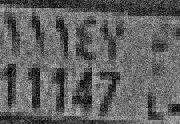
\includegraphics[width=0.3\linewidth]{../assets/gaussian_noise.png}\quad

\includegraphics[width=0.3\linewidth]{../assets/sp_noise.png}\\[2pt]
{\small چپ: تمیز — وسط: نویزِ گاوسی — راست: نمک‌وفلفل (ضربه‌ای)}
\end{center}

\begin{itemize}
  \item \textbf{نویزِ گاوسی}: نوساناتِ تصادفیِ کوچک که به هر پیکسل اضافه می‌شود (نویزِ حسگر/خواندن).
  \item \textbf{نمک‌وفلفل} (ضربه‌ای): پیکسل‌های تصادفیِ گیرکرده روی ۰ یا ۲۵۵ (پیکسلِ مرده، انتقال).
  \item \textbf{پواسون} (شات): از شمارشِ فوتون؛ در نواحیِ تاریک/نورِ کم قوی‌تر.
\end{itemize}

\begin{riyazi}
مدلِ گاوسی: $g = f + n$ با $n\sim\mathcal{N}(0,\sigma^2)$ — جمعی و میانگین‌صفر. یعنی هر پیکسلِ
مشاهده‌شده = پیکسلِ واقعی + یک مقدارِ تصادفیِ کوچک.
\end{riyazi}

\subsection{تولیدِ نویزِ مصنوعی برای آزمایش}

برای فهمِ نویز، بهترین راه ساختنِ آن است. با یک تصویرِ تمیز شروع کنید و نویزِ \emph{معلوم} اضافه
کنید — حالا «حقیقتِ زمینه» دارید و می‌توانید هر حذف‌کننده را عینی بسنجید:

\begin{ltrcode}
\begin{lstlisting}[language=Python]
def add_gaussian(img, sigma=20):
    noise = np.random.normal(0, sigma, img.shape)
    return np.clip(img.astype(np.float32) + noise, 0, 255).astype(np.uint8)

def add_salt_pepper(img, p=0.06):
    out = img.copy()
    out[np.random.rand(*img.shape) < p/2] = 255   # salt
    out[np.random.rand(*img.shape) < p/2] = 0     # pepper
    return out
\end{lstlisting}
\end{ltrcode}

\begin{yaddasht}
این یک تکنیکِ آزمایشیِ کلیدی در پردازش تصویر است: چون معمولاً «تصویرِ واقعیِ بدونِ نویز» را نداریم،
با افزودنِ نویزِ مصنوعی به یک تصویرِ تمیز، یک آزمایشِ کنترل‌شده می‌سازیم. همان کاری که برای تولیدِ
شکل‌های این جلسه کردیم.
\end{yaddasht}

\subsection{تشخیصِ نویز}

به یک ناحیهٔ \textbf{تخت} نگاه کنید: گاوسی = یک پخشِ محو؛ نمک‌وفلفل = لکه‌های سیاه/سفیدِ منزوی.
هیستوگرامِ یک وصلهٔ تخت: گاوسی قله را پهن می‌کند؛ ضربه‌ای پیک‌هایی در ۰ و ۲۵۵ اضافه می‌کند. فیلتر
را با آنچه می‌بینید تطبیق دهید.

\begin{hoshdar}
میانگین‌گیری (تاریِ گاوسی) به‌سختی نمک‌وفلفل را لمس می‌کند — فقط هر لکه را به یک لکهٔ خاکستری
پخش می‌کند. استفاده از فیلترِ اشتباه، بدترین حالت است: هم نویز می‌ماند و هم جزئیات از دست می‌رود.
\end{hoshdar}

% ===================================================================
\section{بازسازی (Restoration)}

\subsection{حذفِ نویزِ گاوسی}

\begin{center}
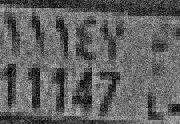
\includegraphics[width=0.23\linewidth]{../assets/gaussian_noise.png}\ %
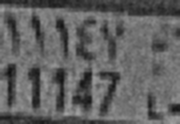
\includegraphics[width=0.23\linewidth]{../assets/gauss_denoise_gauss.png}\ %
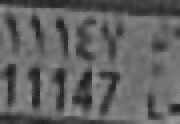
\includegraphics[width=0.23\linewidth]{../assets/gauss_denoise_bilateral.png}\ %
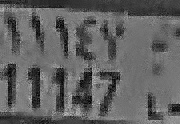
\includegraphics[width=0.23\linewidth]{../assets/gauss_denoise_nlm.png}\\[2pt]
{\small نویزی — تاریِ گاوسی — دوطرفه — میانگینِ ناموضعی (NLM)}
\end{center}

تاریِ گاوسی هموار می‌کند اما لبه‌ها را می‌مالد؛ دوطرفه لبه‌ها را حفظ می‌کند؛ NLM بهترین است اما
کندترین.

\subsection{حذفِ نمک‌وفلفل — میانه برنده است}

\begin{center}

\includegraphics[width=0.3\linewidth]{../assets/sp_noise.png}\quad
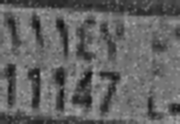
\includegraphics[width=0.3\linewidth]{../assets/sp_denoise_gauss.png}\quad
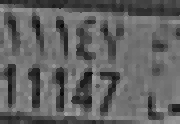
\includegraphics[width=0.3\linewidth]{../assets/sp_denoise_median.png}\\[2pt]
{\small نویزی — گاوسی (بد) — میانه (عالی)}
\end{center}

\begin{riyazi}
میانگینِ $\{100,100,100,255\}$ = ۱۶۴ — پرت‌داده آن را بالا می‌کشد. میانهٔ همان = ۱۰۰ — پرت‌داده
کاملاً نادیده گرفته می‌شود. میانگین‌گیری یک ضربه را \emph{پخش} می‌کند؛ میانه آن را \emph{حذف} می‌کند.
\end{riyazi}

\begin{nokte}
میانه در برابرِ پرت‌داده‌ها مقاوم است؛ میانگین نیست. همین یک واقعیت، کلِ نتیجه را توضیح می‌دهد:
یک لکهٔ ۲۵۵ در میانِ ۱۰۰ها، میانه را تکان نمی‌دهد، پس میانه ضربه را می‌کشد و لبه‌ها را نگه می‌دارد.
\end{nokte}

\subsection{دوطرفه و میانگینِ ناموضعی}

\begin{itemize}
  \item \textbf{دوطرفه} (\lr{bilateral}): فقط همسایه‌های \emph{هم‌شدت} را میانگین می‌گیرد $\rightarrow$ هموارکردنِ تخت‌ها، حفظِ لبه.
  \item \textbf{میانگینِ ناموضعی} (\lr{NLM}): پیکسل‌هایی با \emph{الگوی همسایگیِ} مشابه را — هرجای تصویر — میانگین می‌گیرد.
\end{itemize}

NLM بهترین کیفیت را روی نویزِ گاوسی می‌دهد، به قیمتِ سرعت. برای DocScan: دوطرفه یا NLM پیش از
آستانه‌گذاری، لبه‌های رقم را تیز نگه می‌دارد در حالی که دانه‌بندیِ حسگر را می‌کشد.

% ===================================================================
\section{انواعِ بیشترِ نویز}

فراتر از دو نویزِ اصلی، چند نوعِ دیگر که در عمل می‌بینید:

\begin{center}
\begin{tabular}{>{\raggedright\arraybackslash}p{0.24\linewidth} >{\raggedright\arraybackslash}p{0.66\linewidth}}
\toprule
\textbf{نویز} & \textbf{منشأ و درمان} \\
\midrule
پواسون (شات) & شمارشِ فوتون؛ در نورِ کم بدتر؛ NLM یا پایدارسازیِ واریانس \\
کوانتش & از عمقِ بیتِ پایین (نوارنوارشدن)؛ \lr{dithering} \\
دوره‌ای & الگوی تکرارشونده (تداخلِ الکتریکی، اسکن)؛ حوزهٔ فرکانس (جلسهٔ ۶) \\
لکه‌ای (\lr{speckle}) & ضربی، در راداری/سونوگرافی؛ فیلترهای ویژه \\
\bottomrule
\end{tabular}
\end{center}

\begin{nokte}
نویزِ \textbf{دوره‌ای} برای فیلترهای مکانی نامرئی است — یک الگوی موجیِ منظم را نمی‌توان با
میانگین‌گیریِ محلی حذف کرد، چون در همه‌جا هست. آن را در \emph{حوزهٔ فرکانس} (جلسهٔ ۶) حذف می‌کنیم،
جایی که به‌صورتِ چند نقطهٔ روشن ظاهر می‌شود و می‌توان دقیقاً حذفشان کرد.
\end{nokte}

% ===================================================================
\section{مثالِ عددیِ PSNR}

بیایید PSNR را دستی حساب کنیم تا معنایش روشن شود. فرض کنید دو تصویرِ کوچک داریم که تفاوتشان در
میانگینِ مربعاتِ خطا (\lr{MSE}) برابرِ ۲۵ است (یعنی به‌طورِ متوسط هر پیکسل ۵ واحد خطا دارد):
\[
\mathrm{PSNR} = 10\log_{10}\frac{255^2}{25} = 10\log_{10}(2601) \approx 34.2 \text{ dB}
\]

\textbf{تفسیر:} PSNRِ بالای ۳۰ dB معمولاً کیفیتِ خوب، و بالای ۴۰ dB عالی است. اگر یک حذف‌کنندهٔ
نویز PSNR را از ۲۵ به ۳۴ dB ببرد، بهبودِ چشمگیری داده. اما دقت کنید: PSNR فقط خطای پیکسلی را
می‌سنجد؛ یک تصویرِ کمی تارِ اما «تمیز» ممکن است PSNRِ خوب بگیرد در حالی که ارقام خوانا نیستند —
برای همین SSIM یا دقتِ OCRِ نهایی سنجهٔ بهتری‌اند.

\begin{yaddasht}
درسِ کلی: هیچ سنجهٔ واحدی کامل نیست. PSNR ساده و رایج است، SSIM ادراکی‌تر، و بهترین سنجه اغلب
\textbf{عملکردِ پایین‌دستی} است (آیا OCR بهتر شد؟). برای پروژه، هر سه را در نظر بگیرید.
\end{yaddasht}

% ===================================================================
\section{تمرینِ کلاسیِ وسط‌جلسه (۱۰ دقیقه)}

\begin{tamrin}
برای هر وضعیت، کدام فیلتر و چرا؟ (۱) یک کنتورِ اسکن‌شده با نقاطِ سیاه/سفیدِ تصادفی. (۲) یک عکسِ
موبایلیِ کم‌نور با دانه‌بندیِ ریز در همه‌جا. (۳) سندی که باید لبه‌های متن تیغه‌ای بماند در حالی که
دانه حذف می‌شود. (۴) چطور \emph{اندازه} می‌گیرید که حذفِ نویزتان واقعاً کمک کرد؟
\end{tamrin}

\textbf{جمع‌بندی:} (۱) نمک‌وفلفل $\rightarrow$ \textbf{میانه}. (۲) دانهٔ گاوسی $\rightarrow$
گاوسی/NLM. (۳) حفظِ لبه $\rightarrow$ \textbf{دوطرفه} (یا NLM). (۴) با \textbf{PSNR}/SSIM در برابرِ
مرجعِ تمیز، یا با دقتِ OCRِ نهایی. قاعدهٔ طلایی: \textbf{ارزان‌ترین} فیلتری که نویزِ موردِ اهمیتِ
\emph{خطِ لولهٔ شما} را حذف کند.

% ===================================================================
\section{راهبردِ حذفِ نویز در عمل}

انتخابِ فیلتر تنها بخشِ ماجرا نیست؛ یک راهبردِ کامل:

\begin{enumerate}
  \item \textbf{تشخیص}: به یک ناحیهٔ تخت نگاه کنید و هیستوگرامش را ببینید. گاوسی است یا ضربه‌ای؟
  \item \textbf{انتخابِ فیلتر}: میانه برای ضربه، گاوسی/دوطرفه/NLM برای گاوسی.
  \item \textbf{تنظیمِ قدرت}: از ضعیف شروع کنید و زیاد کنید تا نویز کافی حذف شود — نه بیشتر.
  \item \textbf{اندازه‌گیری}: PSNR (اگر مرجع دارید) یا اثر بر گامِ بعدی (کیفیتِ آستانه).
  \item \textbf{تکرار روی موارد سخت}: پارامترها را روی نویزی‌ترین تصاویر تنظیم کنید، نه تمیزترین.
\end{enumerate}

\begin{ltrcode}
\begin{lstlisting}[language=Python]
# a small experiment: add known noise, denoise, measure
clean = cv2.imread('meter.png', 0)
noisy = add_gaussian(clean, sigma=20)
for f in [cv2.medianBlur, gaussian, bilateral, nlm]:
    out = f(noisy)
    print(f.__name__, psnr(clean, out))   # pick the winner objectively
\end{lstlisting}
\end{ltrcode}

\subsection{ترتیب در خطِ لوله}

جایگاهِ حذفِ نویز در خطِ لوله مهم است: \emph{زود} (پس از خاکستری‌سازی، پیش از بهبود و آستانه).
چرا؟ چون بهبودِ کنتراست (جلسهٔ ۲) نویز را \emph{تقویت} می‌کند، پس اگر اول بهبود دهید و بعد حذفِ
نویز کنید، کارتان سخت‌تر است. و آستانه‌گذاری روی تصویرِ نویزی، لکه‌های سیاه/سفیدِ فراوان می‌سازد.

\begin{nokte}
اما یک استثنا: اگر نویز خیلی کم است، حذفِ نویز ممکن است جزئیاتِ بیشتری از نویز بگیرد. همیشه
بپرسید «آیا واقعاً به حذفِ نویز نیاز دارم؟» — گاهی بهترین حذفِ نویز، هیچ‌حذفِ‌نویز است.
\end{nokte}

% ===================================================================
\section{بخشِ عمیق}

\subsection{اندازه‌گیریِ بازسازی: PSNR و SSIM}

\begin{itemize}
  \item \textbf{PSNR}: بر اساسِ خطای میانگینِ مربعات در برابرِ مرجعِ تمیز؛ بالاتر = نزدیک‌تر (بر حسبِ دسی‌بل).
  \item \textbf{SSIM}: ادراکی — ساختار را مقایسه می‌کند، نه فقط خطای پیکسلی؛ با قضاوتِ انسان بهتر می‌خواند.
\end{itemize}

\begin{riyazi}
$\mathrm{PSNR}=10\log_{10}\dfrac{255^2}{\mathrm{MSE}}$ که در آن \lr{MSE} میانگینِ مربعِ تفاوتِ
دو تصویر است.
\end{riyazi}

اگر مرجعِ تمیز دارید (یا یک آزمایشِ نویزِ مصنوعی)، \emph{اندازه بگیرید}، چشمی قضاوت نکنید. یک
تکنیکِ رایج: یک تصویرِ تمیز بردارید، نویزِ \emph{معلوم} اضافه کنید، حذف کنید، و PSNR را با اصلِ
تمیز بسنجید — چون «حقیقتِ زمینه» را دارید.

\subsection{معضلِ حذفِ نویز}

هر حذف‌کنندهٔ نویز، \textbf{حذفِ نویز} را در برابرِ \textbf{حفظِ جزئیات} معاوضه می‌کند. حذفِ خیلی
کم $\rightarrow$ نویز گامِ بعدی را می‌شکند؛ خیلی زیاد $\rightarrow$ ارقام را پاک می‌کنید. ناهارِ
مجانی وجود ندارد: نقطهٔ کاری را برای هدفِ \emph{خودتان} (ارقامِ خوانا) انتخاب کنید. برای هدفِ
پایین‌دستی حذفِ نویز کنید، اندازه‌گیری‌شده روی تصاویرِ سخت — نه برای زیباترین دیوارِ تخت.

\subsection{بازسازی در برابرِ بهبود}

\textbf{بهبود} (جلسهٔ ۲) تصویر را \emph{بهتر به‌نظر} می‌رساند (ذهنی). \textbf{بازسازی} تلاش می‌کند
با مدل‌کردنِ تخریب، اصل را \emph{بازیابی} کند (عینی). رفعِ تاری (\lr{deblurring}) هم بازسازی است:
اگر تاری را بشناسید (تابعِ پخشِ نقطه، \lr{PSF})، می‌توانید تا حدی معکوسش کنید.

\subsection{رفعِ تاری و PSF}

تاری = کانولوشن با یک \textbf{تابعِ پخشِ نقطه} (\lr{PSF}). رفعِ تاری = واهم‌گشت (\lr{deconvolution}).
معکوسِ ساده‌لوحانه نویز را به‌طورِ فاجعه‌بار تقویت می‌کند؛ روش‌های واقعی (\lr{Wiener},
\lr{Richardson-Lucy}) منظم‌سازی می‌کنند. تاریِ حرکتی/دفوکوس روی عکسِ کنتور اغلب بهتر است
\emph{پرهیز} شود (عکسِ ثابت) تا رفع شود. رفعِ تاریِ کامل وقتی اطلاعات واقعاً از دست رفته ناممکن
است — پیش‌گیری از بازسازی بهتر است.

% ===================================================================
\section{حذفِ نویزِ زمانی و یادگیریِ عمیق}

\subsection{میانگین‌گیریِ چند فریم}

اگر چند عکس از \emph{یک} صحنهٔ ثابت دارید، آن‌ها را میانگین بگیرید: نویز حذف می‌شود، سیگنال
می‌ماند. $N$ فریم نویزِ گاوسی را با $\sqrt{N}$ کاهش می‌دهند — ارزان‌ترین و باکیفیت‌ترین
حذف‌کنندهٔ نویز، بدونِ از‌دست‌رفتنِ جزئیات. برای کنتوری که می‌توانید دوبار عکس بگیرید، این از هر
فیلترِ تک‌تصویری بهتر است.

\begin{yaddasht}
وقتی اکتساب را کنترل می‌کنید، میانگین‌گیریِ یک برستِ عکس بهترین حذفِ نویزی است که می‌توانید انجام
دهید. این یک درسِ کلی است: گاهی بهترین راهِ حلِ یک مسئلهٔ پردازش، بهبودِ \emph{اکتساب} است، نه
پردازشِ سخت‌تر.
\end{yaddasht}

\subsection{ریاضیِ میانگین‌گیریِ فریم‌ها}

چرا میانگین‌گیریِ $N$ فریم نویز را با $\sqrt{N}$ کاهش می‌دهد؟ فرض کنید هر فریم
$g_i = f + n_i$ است که $f$ سیگنالِ ثابت و $n_i$ نویزِ مستقلِ میانگین‌صفر با انحرافِ معیارِ
$\sigma$ است. میانگین:
\[
\bar{g} = \frac{1}{N}\sum_{i=1}^{N} g_i = f + \frac{1}{N}\sum_{i=1}^{N} n_i
\]
جملهٔ سیگنال ($f$) بی‌تغییر می‌ماند، اما انحرافِ معیارِ جملهٔ نویز به $\sigma/\sqrt{N}$ کاهش
می‌یابد (چون نویزها مستقل‌اند و تا حدی همدیگر را خنثی می‌کنند). پس با ۴ فریم، نویز نصف می‌شود؛ با
۱۰۰ فریم، ده برابر کمتر.

\begin{riyazi}
انحرافِ معیارِ نویزِ میانگین‌گرفته‌شده: $\sigma_{\bar{g}} = \dfrac{\sigma}{\sqrt{N}}$. این پایهٔ
ریاضیِ چرا «برستِ عکس» بهترین حذفِ نویز است.
\end{riyazi}

\subsection{نسبتِ سیگنال به نویز (SNR)}

\textbf{SNR} می‌سنجد سیگنال چقدر قوی‌تر از نویز است. SNRِ بالا = تصویرِ تمیز؛ پایین = نویزی. هدفِ
حذفِ نویز، بالابردنِ SNR است بدونِ آسیب به سیگنال. مفهومِ مرتبطی با PSNR است، اما SNR به خودِ
تصویر (نه یک مرجع) اشاره دارد. در عمل، وقتی SNR خیلی پایین باشد (نورِ خیلی کم)، هیچ فیلتری
معجزه نمی‌کند — اطلاعات از ابتدا نبوده. باز هم: کیفیتِ اکتساب مهم‌تر از هر پردازشِ بعدی است.

\subsection{حذف‌کننده‌های یادگیریِ عمیق (پیش‌درآمد)}

حذف‌کننده‌های مدرن، CNNهایی‌اند که روی جفت‌های (نویزی، تمیز) آموزش دیده‌اند — از روش‌های کلاسیک
بهترند. اما به داده، محاسبه نیاز دارند و می‌توانند جزئیاتی را که وجود ندارد \emph{توهم} کنند.

چند نکتهٔ مهم دربارهٔ حذف‌کننده‌های عمیق:

\begin{itemize}
  \item \textbf{مزیت}: کیفیتِ چشمگیر، به‌ویژه روی نویزِ پیچیده و واقعی که مدلِ ریاضیِ ساده‌ای ندارد.
  \item \textbf{هزینه}: نیاز به دیتاستِ آموزشی، GPU، و زمانِ آموزش.
  \item \textbf{خطر}: \textbf{توهم} — شبکه ممکن است جزئیاتی بسازد که «قابلِ‌باور» اما \emph{غلط}‌اند. برای یک کنتور، این فاجعه‌بار است: یک رقمِ ۳ ممکن است به ۸ تبدیل شود!
  \item \textbf{قابلیتِ تفسیر}: برخلافِ میانه (که دقیقاً می‌دانید چه می‌کند)، یک CNN جعبهٔ سیاه است.
\end{itemize}

\begin{hoshdar}
برای کاربردهای حساس مثلِ خواندنِ کنتور، \textbf{توهمِ} حذف‌کننده‌های عمیق خطرِ جدی است. یک روشِ
کلاسیکِ ساده که ممکن است کمی نویز باقی بگذارد، بهتر از یک شبکه‌ای است که با اطمینان رقمِ غلط
می‌سازد. برای DocScan، کلاسیک (میانه/دوطرفه/NLM) معمولاً کافی و کاملاً قابلِ‌تفسیر است.
\end{hoshdar}

% ===================================================================
\section{کور در برابرِ غیرکور}

حذفِ نویز/رفعِ تاری دو حالت دارد: \textbf{غیرکور} (\lr{non-blind}) که در آن پارامترهای تخریب
(مثلِ $\sigma$ نویز یا PSFِ تاری) را می‌دانید، و \textbf{کور} (\lr{blind}) که باید آن‌ها را هم
تخمین بزنید. غیرکور آسان‌تر و دقیق‌تر است؛ کور واقعی‌تر اما سخت‌تر. در عمل، اغلب $\sigma$ نویز را
از یک ناحیهٔ تختِ تصویر تخمین می‌زنیم و مسئله را به غیرکور تبدیل می‌کنیم.

\begin{yaddasht}
برای DocScan، معمولاً حالتِ کور داریم (نمی‌دانیم عکس چقدر نویزی است). یک راهبردِ عملی: چند سطحِ
حذفِ نویز را امتحان کنید و آن را که بهترین باینریِ نهایی را می‌دهد انتخاب کنید — یعنی از هدفِ
پایین‌دستی برای تنظیمِ پارامترِ نامعلوم استفاده کنید.
\end{yaddasht}

% ===================================================================
\section{این جلسه در پروژهٔ نهایی}

در DocScan، حذفِ نویز \emph{زودهنگام} در خطِ لوله می‌آید — پیش از بهبود (که نویز را تقویت می‌کرد)
و پیش از آستانه‌گذاری (که نویز خرابش می‌کرد). اما نه \emph{خیلی} تهاجمی: حذفِ بیش‌ازحد ارقامی را
که لازم دارید پاک می‌کند.

جریانِ عملی برای یک عکسِ کنتورِ نویزی:
\begin{ltrcode}
\begin{lstlisting}[language=Python]
gray  = cv2.cvtColor(img, cv2.COLOR_BGR2GRAY)
den   = cv2.bilateralFilter(gray, 9, 60, 60)   # denoise, keep digit edges
# then: enhance (CLAHE) -> threshold (adaptive) -> morphology (Week 7)
\end{lstlisting}
\end{ltrcode}

\begin{yaddasht}
\textbf{مایلستونِ هفتهٔ ۴:} برای عکس‌های نویزیِ کنتور، نشان دهید که حذفِ نویزِ درست، باینریِ نهایی
(از جلسهٔ ۲) را تمیزتر می‌کند. اگر بدونِ حذفِ نویز آستانه بزنید، نویز به لکه‌های سیاه/سفیدِ فراوان
تبدیل می‌شود که ارقام را غیرقابلِ‌خواندن می‌کند.
\end{yaddasht}

% ===================================================================
\section{جمع‌بندی}

\begin{itemize}
  \item تشخیصِ نویزِ گاوسی در برابرِ ضربه‌ای و نام‌بردنِ منشأِ فیزیکی.
  \item انتخابِ فیلترِ متناظر (میانه / گاوسی / دوطرفه / NLM).
  \item اندازه‌گیریِ بازسازی با PSNR/SSIM به‌جای قضاوتِ چشمی.
  \item استدلال دربارهٔ مبادلهٔ نویز-در-برابرِ-جزئیات برای خطِ لوله.
\end{itemize}

\begin{tamrin}
\textbf{تحویلیِ این هفته (پیش از جلسهٔ ۵):} (۱) نویزِ گاوسی و نمک‌وفلفل به یک کنتورِ تمیز اضافه
کنید (نویزِ معلوم = حقیقتِ زمینه). (۲) هرکدام را با ۳ فیلتر حذف کنید؛ PSNR را در برابرِ اصلِ تمیز
حساب و جدول کنید. (۳) موردی نشان دهید که فیلترِ «اشتباه» شکست می‌خورد (گاوسی روی نمک‌وفلفل). (۴)
DocScan: یک عکسِ نویزیِ واقعی را چنان حذفِ نویز کنید که باینریِ Otsu/تطبیقی‌اش تمیز شود.
\end{tamrin}

\subsection*{نویز چطور هر گام را می‌شکند}

\begin{center}
\begin{tabular}{>{\raggedright\arraybackslash}p{0.3\linewidth} >{\raggedright\arraybackslash}p{0.6\linewidth}}
\toprule
\textbf{گام} & \textbf{اثرِ نویز اگر حذف نشود} \\
\midrule
آستانه‌گذاری & لکه‌های سیاه/سفیدِ فراوان؛ ارقامِ شکسته \\
تشخیصِ لبه (ج۵) & لبه‌های کاذبِ بی‌شمار \\
یافتنِ کانتور (ج۹) & کانتورهای ریزِ نویزی؛ شمارشِ غلط \\
تطبیقِ ویژگی (ج۱۰) & نقاطِ کلیدیِ ناپایدار \\
\bottomrule
\end{tabular}
\end{center}

این جدول توضیح می‌دهد چرا حذفِ نویزِ زودهنگام این‌قدر مهم است: نویز در گام‌های بعدی \emph{تکثیر}
می‌شود و رفعش سخت‌تر می‌گردد.

\subsection*{چک‌لیستِ دام‌های این هفته}

\begin{itemize}
  \item گاوسی روی نمک‌وفلفل (پخشِ لکه‌ها به‌جای حذف) — به‌جایش میانه.
  \item حذفِ نویزِ بیش‌ازحد (پاک‌شدنِ ارقام) — کوچک‌ترین فیلترِ کافی.
  \item بهبود پیش از حذفِ نویز (تقویتِ نویز) — اول حذفِ نویز.
  \item قضاوتِ چشمیِ کیفیت — با PSNR/SSIM یا اثرِ پایین‌دستی اندازه بگیرید.
  \item نادیده‌گرفتنِ نویزِ دوره‌ای در حوزهٔ مکانی — آن را در فرکانس (ج۶) حذف کنید.
\end{itemize}

\subsection*{واژه‌نامهٔ کوتاه}

\begin{center}
\begin{tabular}{>{\raggedright\arraybackslash}p{0.3\linewidth} >{\raggedright\arraybackslash}p{0.6\linewidth}}
\toprule
\textbf{اصطلاح} & \textbf{معنی} \\
\midrule
\lr{Gaussian noise} & نویزِ جمعیِ میانگین‌صفر (حسگر) \\
\lr{Salt-and-pepper} & نویزِ ضربه‌ای (پیکسل‌های ۰/۲۵۵) \\
\lr{Median filter} & میانهٔ همسایگی؛ مقاوم به پرت‌داده \\
\lr{Bilateral / NLM} & حذفِ نویزِ حفظ‌کنندهٔ لبه \\
\lr{PSNR / SSIM} & معیارهای کیفیتِ بازسازی \\
\lr{PSF} & تابعِ پخشِ نقطه (مدلِ تاری) \\
\bottomrule
\end{tabular}
\end{center}

\vspace{0.5cm}
\begin{center}
\textit{فیلتر را با نویز تطبیق بده. میانه برای لکه‌ها، میانگین برای دانه، دوطرفه برای حفظِ لبه.}
\end{center}

\end{document}
